\documentclass[UTF8,12pt,twoside]{article}
\usepackage{ctex}
\usepackage[left=3.18cm,right=3.18cm,top=2.54cm,bottom=2.54cm]{geometry}
\usepackage{amsfonts}
\usepackage{amsmath}
\usepackage{amssymb}
\usepackage{mathtools}
\usepackage{amsthm}
\usepackage{pgfplots}
\usepackage{enumitem}
\usepackage{tikz}
\usepackage{tikz-cd}
\usepackage{changepage}
\usetikzlibrary{arrows}
\usepackage{titlesec}
\usepackage{bm}
\usepackage{graphicx}
\usepackage{cases}
\usepackage{appendix}
\usepackage[colorlinks,linkcolor=black,anchorcolor=black,citecolor=black]{hyperref}
\usepackage[numbers]{natbib}
\usepackage{txfonts}
\usepackage{fancyhdr}


\usepackage{stackengine}
\usepackage{scalerel}
\usepackage{longtable}
\usepackage{multirow,makecell}
\usepackage{multicol}
\usepackage{caption}


%new package
\usepackage{blkarray}


\pagestyle{fancy}
\headheight 27pt
%\fancypagestyle{plain}{}
\fancyhf{}
\fancyhead[CO]{例子与分类定理}
\fancyhead[CE]{例子与分类定理}
\fancyhead[LO,RE]{《蛙鸣》}
\fancyhead[LE,RO]{\thepage}
\usepackage[scaled=0.92]{helvet}	% set Helvetica as the sans-serif font
\renewcommand{\rmdefault}{ptm}		% set Times as the default text font
\bibliographystyle{plain}


\theoremstyle{definition}
\newtheorem{thm}{定理}[section]
\newtheorem{question}{问题}[section]
\newtheorem{assump}[thm]{Assumption}
\newtheorem*{thmm}{定理}  %不带编号
\newtheorem{defn}{定义}[section]
\newtheorem{lem}[thm]{引理}
\newtheorem{prop}[thm]{命题}
\newtheorem*{propp}{命题}%不带编号
\newtheorem{cor}[thm]{推论}
\newtheorem{conj}[thm]{猜想}
\newtheorem*{rmk}{注 }%不带编号
\newtheorem{ex}{例}[section]


\newcommand{\RR}{\mathbb{R}}  %实数
\newcommand{\ZZ}{\mathbb{Z}}  %整数
\newcommand{\NN}{\mathbb{N}}  %自然数
\newcommand{\QQ}{\mathbb{Q}}  %有理数
\newcommand{\CC}{\mathbb{C}}  %复数
\newcommand{\CCt}{\mathbb{C}^{\times}}  %复数
\newcommand{\TT}{\mathbb{T}}  %环面
\newcommand{\PCC}{\mathbb{P}_{\CC}^2} %复射影曲面
\newcommand{\PPC}{\mathbb{P}^1 \times \mathbb{P}^1} %P^1*P^1
\newcommand{\ddiv}{\operatorname{div}} %div
\newcommand{\p}{\partial}  %偏导数
\newcommand{\Img}{\operatorname{Im}}
\newcommand{\GL}{\operatorname{GL}}  
\newcommand{\SL}{\operatorname{SL}}  
\newcommand{\Aut}{\operatorname{Aut}}
\newcommand{\Spec}{\operatorname{Spec}}
\newcommand{\Proj}{\operatorname{Proj}}
\newcommand{\Rep}{\operatorname{Rep}}  
\newcommand{\Pic}{\operatorname{Pic}}
\newcommand{\Nil}{\operatorname{Nil}}
\newcommand{\Sol}{\operatorname{Sol}}
\newcommand{\Alb}{\operatorname{Alb}}
\newcommand{\Coh}{\operatorname{Coh}}
\newcommand{\uniofsl}{\stackon[-4pt]{$\SL_2(\RR)$}{\vstretch{0.75}{\hstretch{1.2}{\widetilde{\phantom{\;\;\;\;\;\;\;\;}}}}}}	%万有覆叠
\newcommand*\extarr{\mathrel{\scalebox{5.0}[1.0]{\hbox{$\rightleftarrows $}}}} %图表箭头


\numberwithin{equation}{section}
\setcounter{tocdepth}{4}
\usepackage{xcolor}
\begin{document}
\title{\textbf{例子与分类定理}}
\author{周潇翔}
%%\and
%%{佚名2}\\{\footnotesize 16级数院}\\{\footnotesize Email: \texttt{12345678@mail.ustc.edu.cn}}
%% }
\date{\today}
\maketitle

\begin{abstract}
	
	
	作为一个偏复代数几何的入门级综述, 这篇文章以分类定理的方式介绍了众多几何对象, 并尝试总结理解这些例子的一套系统方式. 通过这篇文章,我们希望读者: 
	\begin{itemize}
		\setlength{\itemsep}{0pt}
		\setlength{\parsep}{0pt}
		\setlength{\parskip}{0pt}
		\item 了解到分类定理的存在;
		\item 对每个分类定理知道基本的例子;      
		\item 尝试用例子来引导理论知识;
		\item 激发对经典几何理论的兴趣;
		\item 接受自己无法学会所有知识的事实,初学时抓大放小;
		\item 在大框架下提出系统性的问题.
	\end{itemize}
	%这篇文章非原创,也没有创新之处,都是这个领域的人都知道的结论.想借这个机会找人和我一起算算每个例子的不变量.我还想搞一个相关的数据库/或者找一个
\end{abstract}


\section{问题简介}

或许除了Grothendieck以外, 人们很难在没有例子的情况下打磨自己的数学理解. 一个toy example有以下几种蹂躏的方式: 
\begin{itemize}
	\setlength{\itemsep}{0pt}
	\setlength{\parsep}{0pt}
	\setlength{\parskip}{0pt}
	\item 作为反例,划定定理成立的边界;      
	\item 验证满足定理的条件,得到例子上满足的性质(牛刀杀鸡法);      
	\item 代入定理的证明,对特例理解证明过程;%验证自己卡住的部分只是描述上复杂,或是实际上不平凡,或是其中有逻辑漏洞;      
	\item 帮助正确记忆定理(为了考试);      
	\item 对猜想的“逐例”验证. 一般情况下, 要么对此特例成立,要么无法验证.前者缩小了反例的可能范围,而后者则提出比原猜想更弱的子问题;      
	\item 对几何例子,提供并纠正数学工作者的几何直观: 画图,计算例子中的不变量和结构,描述例子的对称性(自同构群),对空间进行几何操作. 
\end{itemize}


遗憾的是, 数学中存在成百上千的例子, 而他们在数学体系中的地位也不尽相同. 在分析中存在大量性质古怪的反例(例如导数在无理点连续而在有理点间断的可微函数, 见\cite{wanglin2014}), 笔者认为这种例子不是数学的主流. 与之相对, 简单深刻的例子也并不少见(例如椭圆曲线), 但初学者往往无法在铺天盖地的例子中细细分辨.再者,单个例子不可能给出理论的全貌,一叶障目容易失去对结构的宏观把握.

分类定理往往能给出一族简单深刻的例子. 有了分类定理, 我们可以按照从简单到复杂的方法论“逐个”讨论范畴中的对象, 把结论做到自己理解的边界. 本文笔者将列出截至目前学过的几何中3个个人认为最为重要的分类定理, 并尽量按照以下步骤阐述: 
\begin{enumerate}
	\setlength{\itemsep}{0pt}
	\setlength{\parsep}{0pt}
	\setlength{\parskip}{0pt}
	\item 给出分类定理中的初始例子;      
	\item 说明刻画的对象和等价关系,必要时介绍分类定理所需要的不变量;      
	\item 阐述分类定理;      
	\item 说明定理中的冗余对象,给出参数空间;
	\item 给出分类定理外的相关信息(和例子).
\end{enumerate}

\section{闭曲面分类定理}
\subsection{初始例子: 紧致无边可定向闭曲面}
众所周知,我们有如下的紧致无边可定向闭曲面: 
\begin{center}
	\begin{tabular}{|c|c|c|c|c|}
		\hline
		g&0&1&2&3	\\
		\hline
		图像&\begin{minipage}[m]{3cm}
			\vspace{1mm}
			\centering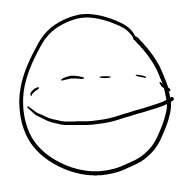
\includegraphics[width=2.5cm]{9-7-fig/genus0.png}
		\end{minipage}&\begin{minipage}[m]{3cm}
			\centering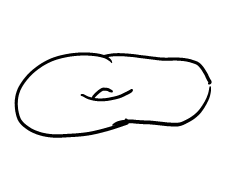
\includegraphics[width=2.7cm]{9-7-fig/genus1.png}
		\end{minipage}&\begin{minipage}[m]{3cm}
			\centering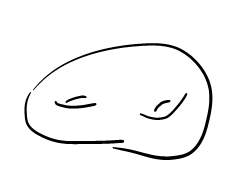
\includegraphics[width=2.8cm]{9-7-fig/genus2.png}
		\end{minipage}&\begin{minipage}[m]{3cm}
			\centering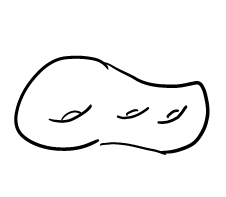
\includegraphics[width=2.7cm]{9-7-fig/genus3.png}
		\end{minipage}	\\
		\hline
	\end{tabular}
\end{center}



我们使用亏格来区分不同的闭曲面.粗略地来说,亏格是指这个曲面的(1维)洞的个数除以2, i.e.,
$$g:=\frac{1}{2}\dim_{\mathbb{R}}H^1(X,\mathbb{R}).\footnote{$\ZZ$系数同调群均定义为奇异同调群, 不过大家几乎不用奇异同调群的定义来计算.}$$
(注意这里的曲面是空心的, 不要忘数“里面的洞”)

对紧致无边可定向曲面来说, 相同亏格的曲面相互之间互相同构. 故而给定某个曲面, 只需算出它的亏格即可理解这个空间的拓扑性质.

对几何空间来说我们总是会算它们的同调群、上同调环、同伦群: 

\begin{figure}[ht]
	\centering
	\begin{tabular}{r|c|c|c|c|c}
		\hline
		$g$&$0$&$1$&$2$&$3$&$4$	\\
		\hline
		$H_0,H^0$&\multicolumn{5}{c}{$\ZZ$}	\\
		\hline
		$H_1,H^1$&$0$ & $\ZZ^2$ &	$\qquad\ZZ^4\qquad$ &$\qquad\ZZ^6\qquad$ &$\ZZ^8$ \\
		\hline
		$H_2,H^2$&\multicolumn{5}{c}{$\ZZ$}	\\
		\hline
		$H^*(M,\ZZ)$& $\ZZ[t]/(t^2)$& $\ZZ\left< x,y\right>/(x^2,y^2,xy+yx)$&\multicolumn{3}{c}{\thead{$\ZZ\left<x_i,y_i\right>/(x_i^2,y_i^2,x_iy_i+y_ix_i,x_iy_i-x_jy_j, $\\\hspace{4.5cm}$x_ix_j,x_iy_j,y_iy_j)$}}\\
		\hline
		$\pi_0(M)$&\multicolumn{5}{c}{$\{*\}$}	\\
		\hline
		$\pi_1(M,x_0)$&$0$ & $\left< x,y \,\middle|\, xyx^{-1}y^{-1} \right>$ &	\multicolumn{3}{c}{$\left< x_i,y_i \,\middle|\, \prod_{i=1}^{n}x_iy_ix^{-1}_iy^{-1}_i \right>$} \\
		\hline
		$\pi_2(M,x_0)$&$\ZZ$& \multicolumn{4}{c}{$0$}	\\
		\hline	
	\end{tabular}
	
\end{figure}

作为计算的副产品, 我们可以得到Betti数和Euler示性数: 
$$b_i:= \dim_{\mathbb{R}}H_i(X,\mathbb{R}), \qquad \chi:= \sum_{n=0}^{2} (-1)^i b_i.$$

对紧致无边可定向闭曲面来说, Euler示性数与亏格之间满足关系
$$\chi=2-2g.$$

\subsection{分类定理}
作为一个简单的推广, 我们去掉可定向和无边的条件. 考虑闭曲面构成的范畴, 等价关系为拓扑空间的同构, 我们有闭曲面分类定理\cite[\href{http://staff.ustc.edu.cn/~wangzuoq/Courses/20S-Topology/Notes/Lec25.pdf}{Lec25}, Theorem 3.2]{wang2021topo}: 

\begin{thm}
	对一个紧的带边曲面$M$, 记$m$为$\p M$连通分支数, 则一定同胚于以下某个曲面挖去$m$个开圆盘: 
	$$S^2, \quad\Sigma_k:= \mathbb{T}^2 \# \cdots \# \mathbb{T}^2,\quad \tilde{\Sigma}_l:=\mathbb{RP}^2 \# \cdots \# \mathbb{RP}^2$$
\end{thm}

通过计算可以得知, $\p M$连通分支数、Euler示性类和可定向性可以唯一确定一个紧带边曲面的结构.

同样的我们可以算它们的同调群、上同调环、同伦群、Betti数和Euler示性数. 当然,一个典范的多边形表示是很好的起点. 这里还可以算两个闭曲面的连通和.

这里的参数空间是$(\mathbb{N} \cup \mathbb{N})\times \mathbb{N}$(作为集合)\footnote{这里的$\mathbb{N} \cup \mathbb{N}$表示无边曲面的参数空间, 最后一个$\mathbb{N}$记录的是$\p M$的连通分支数.}, 连通和给出了参数空间上的幺半群结构.

\subsection{推广: 拓扑流形}
当我们考虑三维或更高维的拓扑流形时, 往往就不再有这样简单的分类定理. 任何一个紧致无边可定向三维拓扑流形可以唯一写成可定向素流形\footnote{我们称三维流形$M$为素流形, 如果不存在不同构于$S^3$的三维流形$M_1,M_2$, 使得$M \cong M_1 \# M_2$.}的连通和\cite{milnor1962unique}. Thurston的几何化猜想(由Perelman于2006年证明, 见\cite{perelman2002entropy,perelman2003ricci})声称我们可以对可定向素流形沿着环面切割, 使得每一块流形都拓扑同胚于以下八种Riemann流形之一的商空间: 
$$S^3,\RR^3,\mathcal{H}^3,S^2 \times \RR, \mathcal{H}^2 \times \RR, \uniofsl,\Nil,\Sol\footnote{关于$\Nil$和$\Sol$的定义详见\cite[p16]{john2014geometrization}, 书中还详尽叙述了这些空间的几何结构.}$$

\begin{figure}[ht]
	\vspace{0cm}
	\centering
	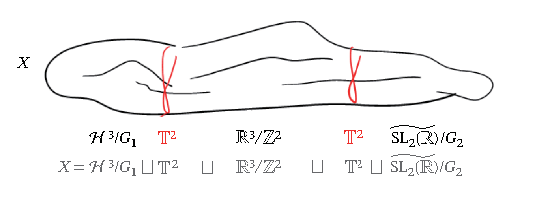
\includegraphics[width=12cm]{9-7-fig/toridecomposition.eps}
	\caption{沿环面切割的示意图}
	\label{fig:toridecomposition}
	
	
\end{figure}

对四维情况, 任何一个有限表示群都可以实现为四维流形的基本群\footnote{参见\url{https://mathoverflow.net/questions/15411}.}, 故分类四维流形的难度比分类有限表示群的难度还大, 可以理解为不可分类. 而对于单连通的紧四维流形, 它的拓扑由相交形式与Kirby–Siebenmann不变量所唯一决定.\footnote{Freedman于1982年在\cite[Theorem 1.5]{freedman1982topology}中给出了单连通的紧四维流形的分类. 关于单连通四维拓扑流形的例子, 可以看\url{http://www.map.mpim-bonn.mpg.de/4-manifolds:_1-connected}和\url{https://en.wikipedia.org/wiki/4-manifold}}%不过人们总是可以划定一个更小的范围来研究.矩阵群、射影代数簇、Grassman流形给出众多性质良好的高维流形的例子,计算拓扑不变量同样是理解这些例子的重要步骤.

在\url{http://www.map.mpim-bonn.mpg.de/}中可以查到大量拓扑流形的相关知识.

\section{复代数曲线的分类}
这节主要参考\cite[Chapter 19]{vakil2017rising},书中总结了技术工具, 然后循序渐进地介绍了各类复代数曲线的性质. 对于复椭圆曲线的解析向处理主要参考\cite[第八章]{Li2019modularform}.

复代数曲线指的是整的光滑射影1维$\CC$-概形(integral smooth projective curve of finite type over $\CC$)\footnote{没学过代数几何的同学可以当成``由代数方程定义的光滑曲线". 另外, 由于复代数曲线和紧黎曼面范畴等价, 大家也可以直接当成紧黎曼面来理解.}. 换句话说,我们考虑的是性质最好的曲线: 没有奇点, 没有素数特征, 解析化后即成为一个紧的黎曼曲面\footnote{黎曼曲面指1维复流形.}. 记$g$为该曲面的亏格,它也可以从层上同调中得到: 
$$g=\dim_{\mathbb{C}}H^1(C,\mathcal{O}_C)=\dim_{\mathbb{C}}H^0(C,\omega_C)$$
这使得我们能够开动层上同调机器来处理曲线. (但是不讲证明的话就可以不用理解层上同调?\footnote{粗略来说,层可以对应流形上的向量丛,给定一个向量丛就得到流形上的一种同调,得到这个流形的一部分信息;      使用不同的层可以得到流形的不同信息.在\cite[Chapter 18]{vakil2017rising}中给出了层上同调的定义、性质以及重要例子.})在闭曲面分类定理给出初步分类后, 我们可以逐亏格地考虑问题.

\subsection{初始例子: 亏格$g=0,1$}
我们在初始例子中考虑亏格$g=0,1$的情况.若$g=0$,则$C \cong \mathbb{P}_{\CC}^1$.

当$g=1$, 事情开始变得复杂起来, 我们不再能单单从它的拓扑中得到它的所有信息(e.g.复结构,概形结构). 幸运的是, 对单个亏格1的复代数曲线$C$, 我们可以用代数机器处理的很干净: 
\begin{itemize}
	\item 固定$C$上一闭点$P$, 则$C$上闭点具有自然的群结构(以$P$为零点), 我们称$(C,P)$为椭圆曲线;      
	\item $\mathbb{P}^2$中的三次光滑超曲面给出了所有亏格1的复代数曲线的例子;      更进一步, 通过变量代换, 每一个亏格1的复代数曲线都对应于一个方程
	$$E_{\lambda}: y^2=x(x-1)(x-\lambda), \qquad \lambda \neq 0,1$$
	
	\item 代数曲线和紧黎曼面具有一一对应的关系, 这样复椭圆曲线对应于亏格1的黎曼面(+点$P$), 同构于$\CC/\Lambda$, 其中$\Lambda$是格点. 这样我们很容易得到复椭圆曲线中的挠点的结构, 群结构也刻画地很清楚;
\end{itemize}

这时我们就可以开始分类亏格1的复代数曲线了. 或者说, 分类所有的复环面$\CC/\Lambda$(在全纯等价的意义下). 复环面之间的同构可以用格点刻画:  $\CC/\Lambda_1 \cong \CC/\Lambda_2$当且仅当存在$\alpha \in \CCt$使得$\Lambda_2=\alpha \Lambda_1$. 这么说来, 复环面的参数空间即为
$$\big\{\,\text{lattices in }  \CC   \,\big\}/\CCt. $$
现在我们要代数化这个空间. 对格点$\Lambda$,取定$\Lambda$的一组基$(z_1,z_2)$\footnote{我们称$(z_1,z_2)$为格点$\Lambda$的基, 若$\Lambda=\ZZ z_1 \oplus \ZZ z_2$.注意格点是几何对象, 同一个格点可以对应不同的基, 不同的基之间相差一个可逆矩阵$M \in \GL_2(\ZZ)$.},则参数空间被代数化为
$$\left\{(z_1,z_2) \in (\CCt)^2\,  \middle|\,z_1,z_2 \;\RR\text{-linear independent, i.e. }\Img \frac{z_1}{z_2} \neq 0 \   \right\} \Big/_{\displaystyle\GL_2(\ZZ)}\,\Big/_{\displaystyle\CCt}$$
现在我们已经得到了参数空间的代数表示, 只不过现在的变量和关系有点多. 当$\Img \frac{z_1}{z_2}<0$时, 通过矩阵$\left(\begin{smallmatrix}
0&1\\ 1 & 0
\end{smallmatrix}\right) \in \GL_2(\ZZ)$交换$z_1$与$z_2$顺序, 这样参数空间简化至
$$\left\{(z_1,z_2) \in (\CCt)^2\,  \middle|\,\Img \frac{z_1}{z_2} > 0 \   \right\} \Big/_{\displaystyle\SL_2(\ZZ)}\,\Big/_{\displaystyle\CCt}$$
这时通过数$\frac{1}{z_2}\in \CCt$的作用,得到参数空间的最终简化版本
$$\left\{(z,1) \in (\CCt)^2\,  \middle|\,\Img z > 0 \   \right\} \Big/_{\displaystyle\SL_2(\ZZ)} \cong \mathcal{H}/{\SL_2(\ZZ)}$$
这个结果令人震惊: 几何对象的参数空间似乎也自然存在着某种几何结构! $\mathcal{H}/\SL_2(\ZZ)$作为拓扑空间同胚于$\CC$, 这意味着“互不同构的复环面大概有$\CC$这么多”. 事实上, 我们有经典的$j$-函数: 
$$j:\left\{ \CC/\Lambda \right\}\!/_{\displaystyle \sim} = \mathcal{H}/{\SL_2(\ZZ)} \longrightarrow \CC \qquad [E_\lambda] \longmapsto \frac{256(\lambda^2-\lambda+1)^3}{\lambda^2(1-\lambda)^2}$$
这给出了复环面和复数的一一对应.

故事至此并没有结束, $\mathcal{H}/{\SL_2(\ZZ)}$背后蕴含着模空间与模形式两大理论, 只是限于笔者学识有限, 力不能及.

\subsection{结构刻画}
鉴于\cite[Chapter 19]{vakil2017rising}已经将低亏格代数曲线的结构处理得很清晰明了, 我们这里只做个简单的总结. 对亏格$g>1$的代数曲线$C$可以分为两类: 超椭圆曲线(hyperelliptic curve)和非超椭圆曲线(non-hyperelliptic curve). 当$C$为超椭圆曲线时, 存在degree为2的分歧映射$\pi: C \longrightarrow \mathbb{P}_{\CC}^1$,有$2g+2$个分歧点, 对应的典范丛$\omega \cong \left(\pi^{-1} \mathcal{O}_{\mathbb{P}_{\CC}^1} (1) \right)^{\otimes (g-1)}$; 当$C$不为超椭圆曲线时, 典范丛$\omega_C$给出$C$至$\mathbb{P}^{g-1}$的射影嵌入. 我们记$\mathbb{P}^n_{a_1,\ldots a_{n-1}}$为$\mathbb{P}^n$中$n-1$个超曲面(次数分别为$a_1,\ldots a_{n-1}$)截出来的曲线, 例如$\mathbb{P}^3_{2,3}$为$\mathbb{P}^3$中的2次曲面和3次曲面截出来的6次曲线.
\begin{center}
	\begin{tabular}{|c|c|c|c|c|c|}
		\hline
		$g$ & 2 & 3 & 4 & 5 & $\geqslant$6 \\
		\hline
		hyperelliptic & dim=3 & dim=5 & dim=7 & dim=9 & dim=2g-1 \\
		\hline
		\multirow{3}*{non-hyperelliptic} & \multirow{3}*{non-exist} & \multirow{2}*{$\mathbb{P}^2_4$: trigonal} & \multirow{2}*{$\mathbb{P}^3_{2,3}$} & dense:$\,\mathbb{P}^4_{2,2,2}$ & not a complete\\
		& &  & & others: trigonal &  intersection \\
		& & dim=6 & dim=9 & dim=12 & dim=3g-3 \\
		\hline 
	\end{tabular}
\end{center}

当然这里还有细节亟待解决. 如何定义``亏格为$g$的代数曲线的模空间" $\mathcal{M}_g$? 如何定义它的维数? 如何将其紧化, 紧化后怎样刻画模空间的结构? 这些问题都可以在\cite{Schm2021moduli}中找到初步的处理及更进一步的参考文献.

\subsection{推广: 带奇点曲线}
由于即使是光滑的复代数曲面也可能有带奇点的1维子簇, 因此在进入下一节之前, 我们有必要提及一些带奇点曲线的性质. 奇点是局部现象, 大家见到的第一个奇点应该是在仿射代数曲线$y^2=x^2(x+1)$和$y^2=x^3$中, 这两条曲线的图像给出了奇点的初始直观. 我们可以定义不同类型的奇点\cite[29.3]{vakil2017rising}, 可以通过各种手段消解奇点(如正规化(normalization))\cite{kollar2009lectures}, 消解过程中几何亏格$p_g(C):=h^0(\tilde{C},\Omega_{\tilde{C}})$不变而代数亏格$g_a(C):=\chi(\mathcal{O}_C)-1$变小. 例如, 退化的椭圆曲线$y^2z=x^3$在$[0: 0: 1]$处有一个奇点, 几何亏格为0而算术亏格为1.

另外值得一提的是, 代数数论中的代数整数环$\mathcal{O}_K$可以视作仿射代数曲线(over $\Spec \ZZ$)上的结构层, 因此代数数论可以视作对某一类特殊代数曲线的研究.

\section{复代数曲面的分类: Enriques–Kodaira classification}
该节主要参考\cite{beauville1996complex}, 在\cite{hartshorne2013algebraic}里面也有一章来介绍,在\cite{vakil2017rising}中则是零零散散地出现相关结论. 由于科普的原因, 笔者打算在介绍最基本的曲面例子的过程中以不严谨的方式介绍代数曲面中的一些概念和相关结论, 之后再简要叙述分类及各类曲面的性质. 在这之前我打算简要总结下我所知的代数曲面中的不变量,初识代数曲面的同学请\textbf{直接跳过}不变量这一小节. \footnote{然而就算对最简单的空间$\mathbb{P}^2_{\CC}$,我也没算出全部的不变量. 希望能有个数据库给出目前已知的所有结论.}

与复代数曲线的定义类似, (复)代数曲面指的是整的光滑射影2维$\CC$-概形(integral smooth projective surface of finite type over $\CC$). 没学过代数几何的同学可以当成``由代数方程定义的光滑曲面".
\setcounter{subsection}{-1}
\subsection{代数曲面的不变量}

分类可以说就是在找不变量, 不变量是分辨不同空间的有力手段, 是反映空间结构的利器. 那么, 对代数曲面, 我们大致按照计算难度从高至低将不变量列举如下: 

\textbf{4.0.1}  首先是以Hodge菱形为代表的数值不变量, 如图所示\footnote{这里$h^{i,j}:=h^j(X,\Omega_{X}^{i})$; 由于对复\textbf{代数}曲面的Hodge菱形上下左右对称, 不同的书上会把$h^{i,j}$放在不一样的位置.这里放置的位置是为了作图的方便.}: 

\begin{figure}[ht]
	\vspace{0cm}
	\centering
	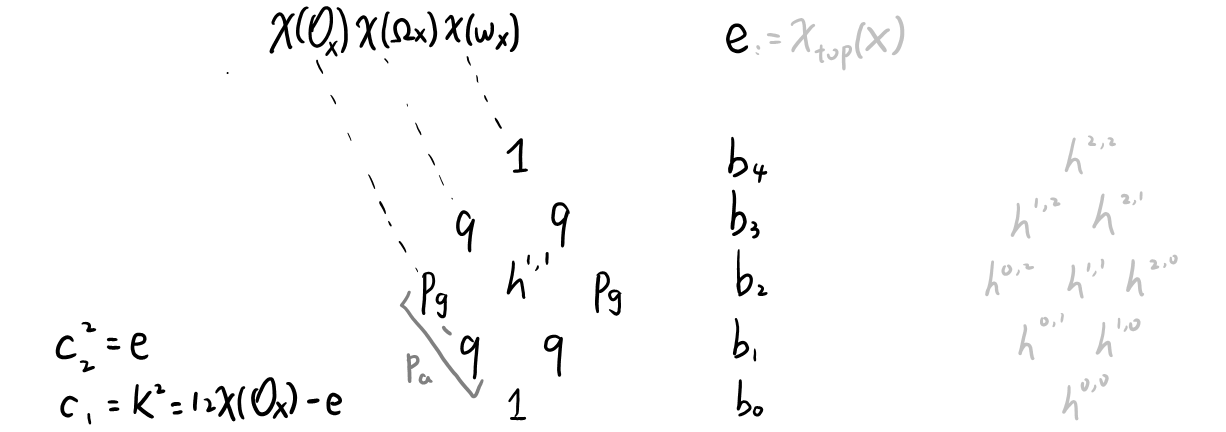
\includegraphics[width=12cm]{9-7-fig/numinv.png}
	\label{fig:numinv}
\end{figure}

注意这里的$q,p_g$为双有理不变量而$h^{1,1}$不是, 其他的不变量全都是$1,q,p_g,h^{1,1}$的线性组合. 在这之外还有新的两个重要的双有理不变量\footnote{注意! 当$n<0$时$h^0(X,\omega_X^{\otimes n})$并不为双有理不变量!}: 
\begin{equation*}
\begin{aligned}
P_n:=&\;h^0(X,\omega_X^{\otimes n}) \qquad \text{ for } n \geqslant 0\\
\kappa:=& \begin{cases}
-\infty, & \text{if }P_n \equiv 0 \text{ for all } n \geqslant 1;\\
\min \left\{ k \in \NN_{\geqslant 0} \,\middle|\, P_n/n^k \text{ is bounded} \right\},& \text{otherwise.}
\end{cases}
\end{aligned}
\end{equation*}
我们称$P_n$为多亏格(plurigenus), $P_1=p_g$为几何亏格(geometric genus), $\chi(\mathcal{O}_X)-1=p_g-q$为算术亏格; $ \kappa$为Kodaira维数, 可以证明$\kappa$只能取$-\infty,0,1,2$这四个值. 这一部分的信息是代数曲面中的基础信息,可以在这个数据库中找到:\url{https://superficie.info/}.

\textbf{4.0.2} 然后是以Picard群为代表的(线)丛的信息.

$$\mathrm{Filtration: }\qquad
\mathrm{P}\underbracket{\underbracket{\!\mathrm{ic}^{\!\!\phantom{0}}  X\overset{\textcolor[RGB]{102,102,102}{\mathbb{Z}^{\,\rho (X)}}}{\supset }\mathrm{Pic}^{\tau}}_{N^1(X)}X
	\overset{\textcolor[RGB]{102,102,102}{torsion}}{\supset}\mathrm{Pic}^0}_{NS(X)}X\overset{\textcolor[RGB]{102,102,102}{scheme}}{\supset}0
$$


该图最清楚的科普/解释是在\cite[18.4.10(with 24.7.5)]{vakil2017rising}(或者说这个图就是这段话的图示). 在搞定Picard群后\footnote{比如,找出$N^1(X)$的生成元.}, 我们有两个方向的延拓: 一方面, 我们可以计算Grothendieck群$K_0(X)$和Chow环$CH^*(X)$; 另一方面, 在$N^1(X)\cong \ZZ^{\rho(X)}$上有自然的双线性型, 是由$\Pic X$上的相交形式
$$\Pic X \times \Pic X \longrightarrow \ZZ \qquad (\mathcal{L}_1,\mathcal{L}_2) \longmapsto \chi(\mathcal{O}_X)-\chi(\mathcal{L}_1^{\bigvee})-\chi(\mathcal{L}_2^{\bigvee})+\chi(\mathcal{L}_1^{\bigvee} \otimes \mathcal{L}_1^{\bigvee})$$
诱导的, 称作相交矩阵. 利用这个相交矩阵, 我们常常可以算出哪些线丛是ample的,哪些线丛是nef的(nef cone),哪些线丛是effective的(effective cone). 当然我们也希望能算出哪些线丛是very ample的, 不过这个难度就高出不少. 我们也关注特殊的线丛, 尤其是典范线丛$\omega_X$\footnote{有些书中也记作$K_X$. 该向量丛在Serre对偶中出现, 是上同调机器里很重要的一个概念}.

\begin{figure}[ht]
	\vspace{0cm}
	\centering
	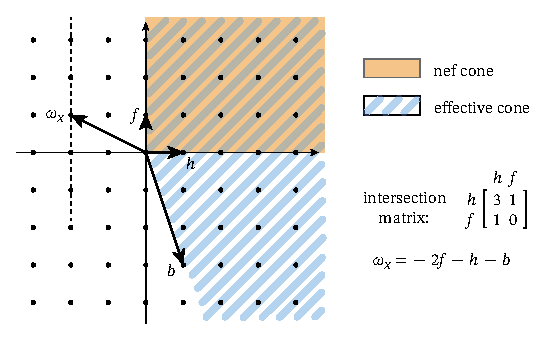
\includegraphics[width=12cm]{9-7-fig/picofF385.eps}
	\label{fig:PicofF3}
	\captionsetup{labelformat=empty}
	\caption{e.g. Informations of $\mathbb{F}_3$ related to its Picard group}
\end{figure}


\textbf{4.0.3} 再接着是代数拓扑中的不变量.

经典的群$\pi_1(X_{\CC}),\pi_n(X_{\CC}),H_n(X_{\CC},\ZZ),H^n(X_{\CC},\ZZ)$自然是计划中的一部分. 而单单视作概形, 我们也有类比的代数基本群(algebraic fundamental group)\footnote{Galois cover的定义, 参见\url{https://en.wikipedia.org/wiki/\%C3\%89tale_fundamental_group}. 这个定义使我们即使在更一般的概形中也能谈论“基本群”, 尽管对于复代数曲面,代数基本群并不能给出比$\pi_1(X)$更多的信息.}:
$$\pi_1^{\text{ét}}(X):=\varprojlim_{\substack{X_i\rightarrow X \\ \text{Gal cover} }} \Aut_X(X_i)$$

提到这里, 我们也会关注$X$的自同构群$\Aut X$. 谈论自同构时请务必小心: 我们的态射是双有理映射(birational map)还是作为概形的同态(morphism)? 当$X$是某条曲线$C$上的纤维丛时, 态射还可能只是丛同态. 提到群作用就有商空间的问题, 不过商空间的理论难度过高, 这里略去不提.

同调代数中的导出范畴相比于层上同调给出了更多的信息,能进行更多操作,是更加自然的研究对象.人们关注$X$的有界导出范畴$\mathcal{D}^b(X):= \mathcal{D}^b(\Coh(X))$的结构\cite[Theorem 6.1]{sosnatriangulated};特别地,也关注$\mathcal{D}^b(X)$作为三角范畴的自同构群\cite[Theorem 8.1,8.3,9.9]{sosnatriangulated}.这些结论与表示论、同调镜像对称有着极为深刻的联系.

我们也关注各种示性类, 不过对复向量丛来说, 一个Chern类就可以推出其它的示性类. 简记$X:=X_{\CC}$,固定$X$上的一个rank为$r$的复向量丛$E$(例如切丛$T_X$).\footnote{Chern类、Todd类的定义可参考\cite[Class 18]{vakil2004algsurf},其 他示性类的一般定义请参考wiki. 这里只给出限定在代数曲面上的公式.}\footnote{在下述 五行中, 这些示性类中简记$c_i:=c_i(E)$, 请勿与陈数混淆.} 

\begin{equation*}
\begin{aligned}
\text{Chern class}& & & c_i(E) & \in H^{2i}(X,\ZZ) \\
\text{Todd class}& & &td(E)=1+\frac{1}{2}c_1+\frac{1}{12}(c_1^2+c_2) & \in H^{2*}(X,\QQ) \\
\text{Stiefel-Whitney class}& & &w(E)=1+c_1+c_2 & \in H^{*}(X,\mathbb{F}_2) \\
\text{Pontryagin class}& & &p(E)=1+c_1^2-2c_2 & \in H^{4*}(X,\ZZ) \\
\text{Euler class}& & &e(E)=c_r(E) & \in H^{2r}(X,\ZZ) \\
\end{aligned}
\end{equation*}

在这里补充一下0.1中的两个陈数(Chern number)的定义: 
$$c_1^2:=c_1(T_X) \cup c_1(T_X) \in H^4(X,\ZZ) \cong \ZZ \qquad c_2:=c_2(T_X) \in H^4(X,\ZZ) \cong \ZZ$$

\textbf{4.0.4} 最后是无法被分到前面三类的相关信息.

所有的光滑射影簇(over $\CC$)都可以视作Kähler流形, 那么代数曲面自然也不例外, 我们有相容的复结构、辛结构和Riemann度量, 有曲率和特殊的Levi-Civita联络, 有$X$上的微分算子层$D_X$和$D_X$-模结构. 这是复流形的视角.

固定$X$上的一个very ample bundle $\mathcal{L}$, 即对应一个闭嵌入(closed embedding)$X \hookrightarrow \mathbb{P}^n$, 我们想知道$X$在这个闭嵌入下的方程、还有$X$中的直线、二次曲线.这是古典代数几何的视角.

另外 ,固定曲面$X$上的一个点$P$, 则$(X,P)$对应于一个Abelian簇$\Alb(X)$, 称作Albanese簇. 我们有典范映射$\alpha:X \longrightarrow \Alb(X)$. 这个簇和映射在代数曲面许多结论的证明中起到了作用.

\subsection{初始例子: 有理曲面}

鉴于大部分没学过代数几何的同学对代数曲面基本没有了解, 我们在这里将花比较大的篇幅来刻画代数曲面最简单的一个例子\footnote{在双有理等价的意义下, 确实是\textbf{一个}例子.}, 并且将$X$和它对应的复曲面$X_{an}$混淆起来. 本节的流程图如下: 



例子\quad \framebox{$\mathbb{P}^2$\quad \quad\quad\quad $\mathbb{P}^1\times\mathbb{P}^1$\quad \quad Hirzebruch曲面
	$\quad \quad \mathbb{P}_3^3$\textcolor[RGB]{102,102,102}{(3次曲面)}}  \textcolor[RGB]{102,102,102}{ {\Big\}} 有理曲面}

$\quad\quad\quad\quad\searrow\quad\quad\quad\nearrow\quad\quad\searrow \quad\quad\nearrow\quad\quad\quad\quad
\searrow\quad\quad\quad \nearrow $

理论\quad\quad\quad\; $\mathrm{Pic}X$\quad\quad\quad\;\; 直纹面\quad\quad\quad\quad\, 双有理等价

\quad\quad\quad\quad\;
相交矩阵\quad\quad\quad\quad\quad\quad\quad\quad\quad\quad\quad blow up



想必复几何中第一个紧复流形的例子一定是复射影空间$\mathbb{CP}^n$, 那么第一个代数曲面的例子自然是二维复射影空间
$$\PCC:= \Proj \CC[x_0,x_1,x_2], $$
它的解析化就是$\mathbb{CP}^2$.我喜欢画一个$S^2$作为$\PCC$的几何直观, 尽管这不完美: $\PCC$是一个复$2$维, 实$4$维的对象, 另外$\PCC$上的两条直线只交于一点, 而$S^2$上两个大圆必交于2点\footnote{$\PCC$上的直线指的是一个一次齐次方程确定的零点集, 例如$[L:x_0+2x_1-4x_2=0]$就是其中的一条直线.}. 你可以用这些小结论来修正你的几何直观.

利用切除正合列(excision exact sequence)\cite[14.2.8]{vakil2017rising}, 我们可以算出$\PCC$的Picard群\footnote{所有的线丛在张量的运算下构成一个群, 称为Picard群. 线丛直观来讲是秩为1的复向量丛, 不过代数几何中更多指的是$X$上秩为1的局部常值层.}
$$\varphi: \Pic \PCC \cong \ZZ$$
对$n \in \ZZ$,记$\mathcal{O}_{\PCC}(n):=\varphi^{-1}(n)$.我们有多种线丛的理解方式\cite[14.1,14.2,15.2]{vakil2017rising}: 
\begin{itemize}
	
	\item 固定$\PCC$上的标准仿射开覆盖$U_0=\Spec k[x_{1/0},x_{2/0}],U_1,U_2$, 我们用转移函数定义线丛$\mathcal{L}_n$, 例如:
	
	\begin{center}
		\begin{tikzcd}
			{\mathbb{C}[x_{1/0},x_{2/0}]} \arrow[rr, "\cdot\;\times x_{0/1}^n", bend left] &  & {\mathbb{C}[x_{0/1},x_{2/1}]} \arrow[ll, "\cdot\;\times x_{1/0}^n", bend left, shift right]
		\end{tikzcd}	
	\end{center}
	
	
	
	其中映射在
	$$U_0 \cap U_1= \Spec k[x_{1/0},x_{2/0}]_{(x_{1/0})}=\Spec k[x_{0/1},x_{2/1}]_{(x_{0/1})}$$
	上定义,我们有$\mathcal{L}_n \cong \mathcal{O}_{\PCC}(n)$.
	
	
	这种方式容易证明是线丛(局部平凡性+转移函数), 问题在于不容易描述全局截影, 给出的解答往往是局部的.
	\item 取超曲面截影$H: x_0=0$, 则$\mathcal{O}_{\PCC}(n)=\mathcal{O}_{\PCC}(nH)$, 其中
	$$\left[\mathcal{O}_{\PCC}(nH)\right](U)=\left\{ t \in K(\PCC)^{\times}: \ddiv|_U t \geqslant -nH  \right\} \cup \{0  \}$$
	这种方式容易描述线丛上的截影, 不过思考的时候需要做一个twist, 有点转换参考系的感觉\footnote{例如, 同样一个有理函数$t \in K(\PCC)^{\times}$, 作为$\mathcal{O}_{\PCC}(nH)$和$\mathcal{O}_{\PCC}(mH)$上的有理截影, 对应的除子就不一致. ($n\neq m$)}. 另外, 这种方式暗示了``线丛对应曲线"的思维方式, 曲线的相交数由此转化为Picard群上的双线性型.
	\item 通过拉回映射, $\PCC$上的线丛可视作$\CC^3 \setminus \left\{ 0 \right\}$上带$\CC^{\times}$-作用的等变线丛.
	
	固定$\CC^{\times}$的$1$维表示$(\lambda,\CC_{\lambda}) \in \Rep(\CC^{\times})$如下:
	$$\lambda: \CC^{\times} \longrightarrow \Aut_{\CC_{\lambda}}(\CC) =\CC^{\times} \qquad t \longmapsto t^{\textcolor{red}{-n}}$$
	$$\CC^{\times} \times \CC_{\lambda} \longrightarrow \CC_{\lambda} \qquad (t,v) \longmapsto \lambda(t)v$$
	另外定义$\CC^{\times}$在$\CC^3 \setminus \left\{ 0 \right\}$右方的左作用\footnote{一般而言大家习惯将群作用实现为左作用,在右方作用是为了实现类似张量积的效果.\\考虑$\CC^{\times}$ 在乘积空间$(\CC^3 \setminus \left\{ 0 \right\}) \times \CC_{\lambda}$上的作用,形式上这是对角作用$$t.(x,v)=(t.x,t.v)$$
	而直观上看却是``将左边的元素移至右边":$$t.(x,v)=(xt^{-1},tv)$$
	这使得商空间看上去更加自然.}
	$$\CC^{\times} \times (\CC^3 \setminus \left\{ 0 \right\}) \longrightarrow \CC^3 \setminus \left\{ 0 \right\} \qquad \big( t,(x_0,x_1,x_2) \big) \longmapsto (x_0t^{-1},x_1t^{-1},x_2t^{-1})$$
	我们得到$\PCC$上的线丛(的复点)
	$$(\CC^3 \setminus \left\{ 0 \right\}) \times^{\CC^{\times}} \CC_{\lambda}:=(\CC^3 \setminus \left\{ 0 \right\}) \times \CC_{\lambda} \;\big/_{\displaystyle \CC^{\times}\text{-action}}$$
	下面的交换图表清晰地显示了不同空间之间的关系:
% https://q.uiver.app/?q=WzAsNCxbMSwwLCIoXFxDQ14zIFxcc2V0bWludXMgXFxsZWZ0XFx7IDAgXFxyaWdodFxcfSkgXFx0aW1lc157XFxDQ157XFx0aW1lc319IFxcQ0Nfe1xcbGFtYmRhfSJdLFswLDAsIihcXENDXjMgXFxzZXRtaW51cyBcXGxlZnRcXHsgMCBcXHJpZ2h0XFx9KSBcXHRpbWVzIFxcQ0Nfe1xcbGFtYmRhfSJdLFswLDEsIlxcQ0NeMyBcXHNldG1pbnVzIFxcbGVmdFxceyAwIFxccmlnaHRcXH0iXSxbMSwxLCJcXFBDQyJdLFsyLDMsIiIsMCx7InN0eWxlIjp7ImhlYWQiOnsibmFtZSI6ImVwaSJ9fX1dLFswLDMsIlxccGkiLDAseyJzdHlsZSI6eyJoZWFkIjp7Im5hbWUiOiJlcGkifX19XSxbMSwwLCIiLDIseyJzdHlsZSI6eyJoZWFkIjp7Im5hbWUiOiJlcGkifX19XSxbMSwyLCIiLDAseyJzdHlsZSI6eyJoZWFkIjp7Im5hbWUiOiJlcGkifX19XV0=
\[\begin{tikzcd}[ampersand replacement=\&]
	{(\CC^3 \setminus \left\{ 0 \right\}) \times \CC_{\lambda}} \& {(\CC^3 \setminus \left\{ 0 \right\}) \times^{\CC^{\times}} \CC_{\lambda}} \\
	{\CC^3 \setminus \left\{ 0 \right\}} \& \PCC
	\arrow[two heads, from=2-1, to=2-2]
	\arrow["\pi", two heads, from=1-2, to=2-2]
	\arrow[two heads, from=1-1, to=1-2]
	\arrow[two heads, from=1-1, to=2-1]
\end{tikzcd}\]
	可以通过局部坐标卡的计算证明
	$$(\CC^3 \setminus \left\{ 0 \right\}) \times^{\CC^{\times}} \CC_{\lambda} = \left(\Spec \mathcal{O}_{\PCC}(n)\right) (\CC) \qquad \mathcal{O}_{\PCC}(n) \cong \pi_* \mathcal{O}_{(\CC^3 \setminus \left\{ 0 \right\}) \times^{\CC^{\times}} \CC_{\lambda}}$$
	
	这种方式与表示论联系密切,给出了一个不依赖于坐标的整体描述,也容易推广构造旗簇(flag variety)上的等变向量丛.只可惜这种方式和其他理解方式之间的转换较为复杂.
	\item 记分次环$S_{\bullet}:=\CC[x_0,x_1,x_2]$,分次$S_{\bullet}$-模$S(n)_{\bullet}:=S_{n+\bullet}$, 则拟凝聚层$\mathcal{O}_{\PCC}(n)=\tilde{S(n)_{\bullet}}$为$\PCC=\Proj S_{\bullet}$上的线丛.
	
	这种方式最为抽象, 但是是一个整体描述, 不依赖于$\PCC$上的坐标, 也容易给出不同线丛之间的映射.
\end{itemize}

理解了$\PCC$上的线丛后, 运用$dx_{1/0}\wedge dx_{2/0} = x_{0/1}^{-3}dx_{2/1} \wedge dx_{0/1}$, 我们可以算出$\omega_{\PCC} \cong \mathcal{O}_{\PCC} (-3)$; 另外, 可直接计算出$\PCC$上的层上同调\cite[18.1.3]{vakil2017rising}: 

$$\dim_{\CC}H^n\left(\PCC,\mathcal{O}_{\PCC}(m)\right)=\begin{cases}
\binom{m+2}{2},& n=0, m\geqslant 0\\
\binom{-m-1}{2}, & n=2,m \leqslant -3\\
0,& \text{otherwise.}
\end{cases}$$

结合$H^2(\PCC,\CC)=\CC$, 我们得到$\PCC$的Hodge菱形: 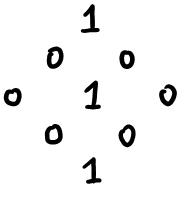
\includegraphics[width=2cm]{9-7-fig/hodgeofp2.png}


我们想知道$\PCC$中曲线的相交情况.事实上,这是著名的\textbf{B\'ezout定理}:

\begin{thm}[B\'ezout Theorem for plane curves, see {\cite[18.6.K]{vakil2017rising}}]
	对$\PCC$上的$m$次曲线$C$和$n$次曲线$C'$, 若$C$与$C'$没有公共分支, 则在计重数的意义下交于$mn$个点.
\end{thm}

这样的结论看上去似乎很难推广至其他代数曲面上, 这敦促我们寻找新的观点. 对代数曲面$X$及其上线丛$\mathcal{L}$, 定义$\chi(\mathcal{L}):=\sum_{n=0}^{\infty}\dim_{\CC} H^n(X,\mathcal{L})$ 以及Picard群上的双线性型
$$(-,-):\Pic X \times \Pic X \longrightarrow \ZZ \qquad (\mathcal{L}_1,\mathcal{L}_2):=\chi(\mathcal{O}_X)-\chi(\mathcal{L}_1^{\wedge})-\chi(\mathcal{L}_2^{\wedge})+\chi(\mathcal{L}_1^{\wedge}\otimes \mathcal{L}_2^{\wedge}), $$
这个双线性型恰好刻画了$X$中曲线的相交数: 可以证明, 对$X$中不可约曲线$C_1,C_2(C_1 \neq C_2)$, $C_1$与$C_2$的相交数(计重数)即为$(\mathcal{O}_X(C_1),\mathcal{O}_X(C_2))$.

这个推广有诸多不平凡之处. 首先, 它给出了不可约曲线$C$的\textbf{自相交数}(self-intersection number): 
$$C^2:=(\mathcal{O}_X(C),\mathcal{O}_X(C))$$
在某些例子的计算中, 曲线的自相交数可能为负数!

其次, 若两个除子$D_1,D_2$\footnote{除子不过是不可约曲线的线性组合, 除子和除子的相交数不过是曲线相交数的线性延拓;      也可以直接将除子$D$视作Picard群中的元素$\mathcal{O}_X(D)$, 简记$D_1 \cdot D_2:= (\mathcal{O}_X(D_1),\mathcal{O}_X(D_2))$.}线性等价(i.e. $\mathcal{O}_X(D_1) \cong \mathcal{O}_X(D_2)$ in $\Pic X$), 则计算相交数(特别是自相交数)时, 我们可以用$D_2$替换$D_1$. 例如$H_0:x_0=0$与$H_1:x_1=0$线性等价($\mathcal{O}_{\PCC}(H_0), \mathcal{O}_{\PCC}(H_1) \cong \mathcal{O}_{\PCC}(1)$), 那么$H_0^2=H_0H_1=1$.

再者, 当$\Pic(X) \cong \ZZ^r$时\footnote{对一般情况, $\Pic X$上的相交形式可以下降(descent)至$N^1(X) \cong \ZZ^{\rho(X)}$,同样是一个有限维矩阵即可搞定.}, 它将代数曲面相交理论的信息浓缩至一个$r \times r$的矩阵, 称为\textbf{相交矩阵}(intersection matrix), 如下图所示: 

\begin{center}
	\begin{blockarray}{*2c}
		\begin{block}{cc}
			& $H$\\
		\end{block}
		\begin{block}{c[c]}
			$H$ & \;\;1\;\; \\
		\end{block}
	\end{blockarray}\quad\quad
	\begin{blockarray}{*3c}
		\begin{block}{ccc}
			& $h$ & $f$ \\
		\end{block}
		\begin{block}{c[cc]}
			$h$ & \;0 & 1\; \\
			$f$ & \;1 & 0\; \\
		\end{block}
	\end{blockarray}\quad\quad
	\begin{blockarray}{*3c}
		\begin{block}{ccc}
			& $h$ & $f$ \\
		\end{block}
		\begin{block}{c[cc]}
			$h$ & \;n & 1\; \\
			$f$ & \;1 & 0\; \\
		\end{block}
	\end{blockarray}
	
	\quad\quad$\mathbb{P}^2$\quad\quad\;\;\;\quad\quad$\mathbb{P}^1\times\mathbb{P}^1$
	\quad\quad\;\;\;\;\quad\quad\quad$\mathbb{F}_n$\quad\quad\quad
\end{center}


利用这个矩阵和一点小技巧, 我们能快速获取大量曲面信息: 例如, 对$\PCC$上$m$次曲线$C$, 设$C \sim kH$ ($\Pic \PCC \cong \ZZ$), 则
$$k=kH \cdot H = C \cdot H =m, $$
故$C \sim mH$.对$\PCC$上$m$次曲线$C$和$n$次曲线$C'$,则有
$$C \cdot C' = mH \cdot nH = mn(H \cdot H)=mn$$
我们重新证明了B\'ezout定理.

有了好的理论,我们当然想把它应用到别的代数曲面上. 第二个常见的代数曲面是$\mathbb{P}^1 \times \mathbb{P}^1$, 我脑海里想象时是类似$\mathbb{T}^2$的图像. 直积的构造自然诱导两个投影映射$\pi_1,\pi_2: \mathbb{P}^1 \times \mathbb{P}^1 \longrightarrow \mathbb{P}^1$, 观察$\pi_2$, 可以发现每个点的原像都是$\mathbb{P}^1$. 事实上,这是第一个$\mathbb{P}^1$-bundle的例子, 我们也称之为\textbf{直纹面}(geometrically ruled surface).

在科大, 大部分同学都在解几中见过直纹面的例子: 单页双曲面和马鞍面. 这并不是偶然, $\PPC$实际上是$\mathbb{P}_{\CC}^3$中的二次曲面: (验证在$\Img \phi$中, $z_0z_3-z_1z_2=0$)
$$\phi: \PPC \longrightarrow \mathbb{P}_{\CC}^3 \qquad ([x_0,x_1],[y_0,y_1]) \longrightarrow \begin{bmatrix}
x_0y_0 & x_0y_1 \\
x_1y_0 & x_1y_1
\end{bmatrix}$$
这样看来, 单页双曲面和马鞍面其实是$\PPC$在实三维空间中的``影子". 另外, 映射$\phi$也说明$\PPC$是射影簇, 亦即``由代数方程定义的光滑曲面". 利用与$\PCC$类似的手法可以得到$\PPC$的Picard群、层上同调、Hodge菱形、相交矩阵,权且留作习题.

回到直纹面, 代数曲面中底空间是$\mathbb{P}^1$的$\mathbb{P}^1$-bundle可不止$\PPC$一种, 我们统称它们为\textbf{Hirzebruch曲面}. 类比球丛往往是从高一维的向量丛中处理得到($S^n=(\RR^{n+1} \setminus O)/\sim$), $\mathbb{P}^1$-bundle 也是从秩2的向量丛里得到. 幸运的是, 我们有$\mathbb{P}^1$上秩2向量丛的分类, 取
$$\mathbb{F}_n:=\Proj (\mathcal{O}_{\mathbb{P}^1} \oplus \mathcal{O}_{\mathbb{P}^1}(n) ), \qquad n \geqslant 0$$
那么$\mathbb{F}_n$即为所有的Hirzebruch曲面. 可以证明, 当$n \geqslant 1$时, $\mathbb{F}_n$有一个自相交数为$n$的曲线,记为$h$; $\mathbb{F}_n$有一个自相交数为$-n$的曲线, 记为$b$, 这是$\mathbb{F}_n$上唯一有负自相交数的曲线;       $h$和$b$都是典范映射$\mathbb{F}_n \longrightarrow \mathbb{P}^1$的截影, 相互无交, 记典范映射的纤维为$f$, 那么有$h\cdot f= b \cdot f =1, h \cdot b =0$; $\Pic \mathbb{F}_n \cong \ZZ^2$由$h$与$f$生成. 这些信息足够给出Hirzebruch曲面上的相交关系.

在双有理等价的意义下\footnote{双有理等价指的是两个代数曲面在一个(Zariski)开集上同构, 因为有太多太多不同的代数曲面, 更宽松的等价条件可以简化分类的难度.}, 我们称所有和$\PCC$双有理等价的曲面为\textbf{有理曲面}(rational surface). 这些代数曲面可视作同一个曲面\footnote{不严格地说, 他们都有开集$\mathbb{A}_{\CC}^2$, 或者说$\mathbb{C}^2$.}. 双有理等价和blow up这个操作有密切关系\footnote{个人认为blow up只有在算过具体例子之后才能理解.}, 可以说blow up是两个双有理等价的曲面之间的桥梁: 两个曲面之间的双有理映射可以由blow up和blow down(即blow up的逆)的操作联系起来.

$$C\,\textcolor[RGB]{102,102,102}{\leftarrow C_1\rightarrow C_2\rightarrow C_3\leftarrow\cdots\,\,\cdots\rightarrow }\,C'$$

Blow down可以简化曲面的复杂程度. 我们想找某个双有理等价类中比较简单的代表元, 严格说就是不能被blow down的曲面, 称为\textbf{极小曲面}(minimal surface). 可以证明, 一个曲面只能经历有限次的blow down即中止, 那么任意一个曲面一定是某个极小曲面经过有限次blow up得到, 我们由此将焦点关注于极小曲面. 如果曲面是由某个曲面做blow up得到的, 那么这个曲面一定有一条(-1)-curve (指同构于$\mathbb{P}^1$,自相交数为 -1);      反过来, Castelnuovo的著名判别法(Castelnuovo's contractibility criterion)告诉我们, 如果曲面$X$上有(-1)-curve, 那么$X$可以沿着这个(-1)-curve做blow down. 有了这样的极小曲面判别法,我们可以轻而易举地看出Hirzebruch曲面除了$\mathbb{F}_1$以外均为极小曲面, $\mathbb{P}_2$也是极小曲面.可以证明这些曲面构成了极小有理曲面的所有例子. 在这种意义下, 我们理解了所有的有理曲面\footnote{还有一个有趣的有理曲面值得一提, $\mathbb{P}^3$中的三次光滑曲面是由$\PCC$ blow up 6个点得到的, 它上面有经典的27条直线.}.
%现在让我们解释“线丛对应曲线”,并将贝祖定理简化到接近平凡的结论.\footnote{对旧有概念新的认知可能会简化定理的证明,但认知之间的等价性往往并不平凡.}

\subsection{分类定理:部分结论}
有理曲面的例子只是代数曲面万花丛中的一枝. 我们在这里简略叙述部分的Enriques–Kodaira分类定理, 并且略过模空间的陈述. 我们按照Kodaira维数$\kappa$将代数曲面(中的极小曲面)\footnote{当$\kappa\neq-\infty$时, 双有理等价类中只有唯一的极小曲面.}粗略分为4类: 

\begin{itemize}
	\item $\kappa=-\infty$: 除了$\PCC$以外都是某个光滑代数曲线上的$\mathbb{P}^1$-丛, 同一条曲线上的两个$\mathbb{P}^1$-丛双有理等价. 我们称$\kappa=-\infty$的(可能非极小)曲面为ruled surface.
	\item $\kappa=0$: 我们按照Hodge菱形的不同将它们分为四类: 
	
	\begin{figure}[ht]
		\vspace{0cm}
		\centering
		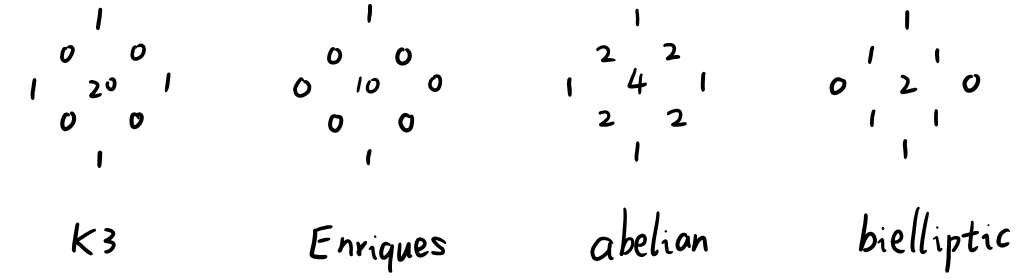
\includegraphics[width=12cm]{9-7-fig/4algsurf.png}
		\label{fig:4algsurf}
	\end{figure}
	
	
	\begin{itemize}
		\item K3曲面\footnote{以三位数学家的名字命名: Kummer,K\"ahler,Kodaira.事实上,还存在非代数的K3曲面.}: 它们的典范丛平凡($\omega_X \cong \mathcal{O}_X$),这是四类曲面中研究得最彻底的曲面.典型例子是$\mathbb{P}^3$中的4次曲面.%事实上,还存在非代数的K3曲面,例如what?
		\item Enriques曲面: 它是某个K3曲面的二次覆叠;      反过来,任给一个K3曲面和$\ZZ/2\ZZ$在其上无固定点的群作用(fixed-point free involution),商空间即是Enrique曲面.典型例子见wiki或者\cite{beauville1996complex}.
		\item 
		Abelian曲面: 它是2维的Abelian簇.典型例子是两个椭圆曲线的乘积$E_1 \times E_2$.
		\item 
		bielliptic曲面: 它一定长成$(E_1 \times E_2) /G$的形式,其中$E_1,E_2$是椭圆曲线, $G$是有限群, 在$E_1$和$E_2$上都有群作用,在$E_1$上是平移作用, 而在$E_2$上的群作用诱导商空间$E_2/G \cong \mathbb{P}^1$. 这类曲面已经有完整的列表, 详见\cite[List VI.20]{beauville1996complex}.
	\end{itemize}
	\item  $\kappa=1$: 这些曲面一定是\textbf{椭圆曲面}(elliptic surface);      存在曲线$C$及映射$\pi:=X\longrightarrow C$使得每个纤维都为椭圆曲线(可能退化). 典型例子是椭圆曲线和亏格大于1的曲线的乘积$E \times C$.
	\item $\kappa=2$: 这类曲面被称为``surfaces of general type", 因为它们到目前为止还没有完全的分类, 只有零零散散的例子. 有一些不等式和等式限制了这类曲面的数值不变量. 典型例子是亏格大于1的两条曲线乘积$C_1 \times C_2$,还有$\mathbb{P}^3$中的$5,~6,~7,\cdots$次曲面.
\end{itemize}

\begin{center}
	\begin{figure}[ht]
		\vspace{0cm}
		\centering
		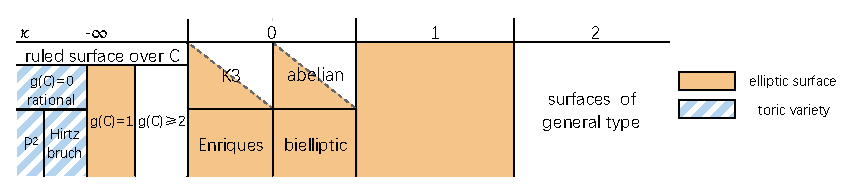
\includegraphics[width=13cm]{9-7-fig/table.eps}
		\label{fig:enrique}
		\captionsetup{labelformat=empty}
		\caption{partial classification(only consider minimal algebraic surface)}
	\end{figure}
\end{center}

\subsection{推广: 复曲面,高维复代数簇}

我们知道复代数曲线与紧Riemann面范畴等价, 但2维情况时, 无脑的类推就不再成立\footnote{由GAGA\cite{serre1956geometrie}, 我们有光滑复射影簇与\textbf{射影}复流形范畴等价, 而一维情况时, 紧Riemann面一定是射影的.}:事实上, 存在2维的紧复流形, 它不能实现为复代数曲面. Hopf曲面就是这样一个例子. 一般的复2维流形会失去许多性质, 例如Hodge菱形的对称性减弱:
\begin{center}
	\begin{figure}[ht]
		\vspace{0cm}
		\centering
		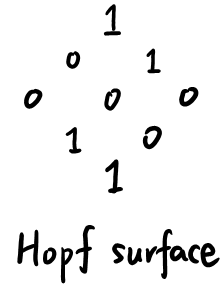
\includegraphics[width=2cm]{9-7-fig/hodgeofhopf.png}
		\label{fig:hodgeofhopf}
	\end{figure}
\end{center}


好消息是,数学上对代数曲面的分类已经推广至一般特征和紧复曲面了,考虑问题时我们仍可以逐个击破\footnote{在这里强烈推荐Kodaira的原始论文\cite{kodaira1964structure,kodaira1966structure,kodaira1968compact,kodaira1968structure}, 其中对每一类曲面(尤其是Hopf曲面)都做了比较细致的刻画, 比如考虑了它们的形变理论.}. 

\begin{center}
	\begin{figure}[ht]
		\vspace{0cm}
		\centering
		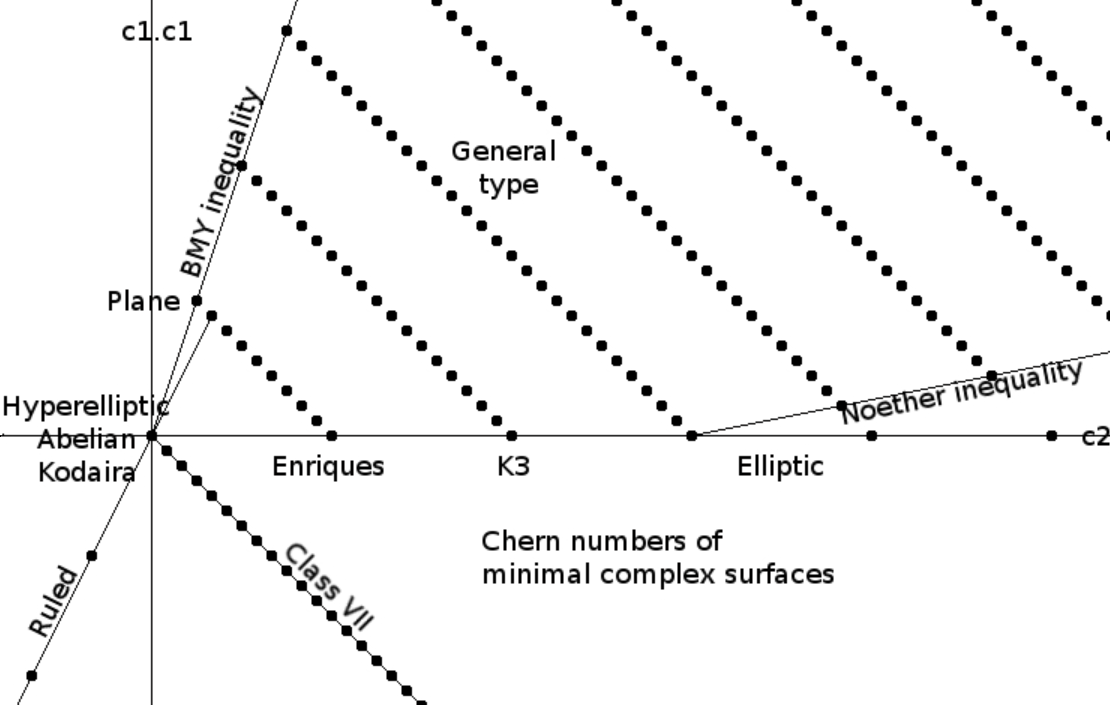
\includegraphics[width=14cm]{9-7-fig/chernofsurfaces.png}
		\label{fig:chernnumber}
		\captionsetup{labelformat=empty}
		\caption{Chern numbers of minimal compact complex surfaces(from wiki)}
	\end{figure}
\end{center}

不过,对于更高维的复代数簇,情况变得更加棘手, 许多公式(如Riemann-Roch公式)由于项数变多不再能发挥出在曲线曲面情形的威力. 不过数学家总能把理论推广到认知的极限,他们划出了多类特殊的代数簇,对每一类代数簇考虑它们的性质:
\begin{center}
	\begin{tabular}{|c|c|}
		\hline
		typical example & Names of variety\\
		\hline
		$\mathbb{P}^n,(\mathbb{P}^1)^n$ & toric variety \\
		\hline
		Grassmannian $Gr(n,r)$ & flag variety\\
		\hline
		$\GL_n(\CC).\SL_n(\CC)$ & group variety\\
		\hline
		$\CC/\Lambda_1 \times\cdots\times \CC/\Lambda_n$ & abelian variety\\
		\hline
	\end{tabular}
\end{center}



\section{总结}


数学问题的无尽性恰如几何空间的无限性. 一个好的理论, 能在这无限的可能中划出一个恰当的边界, 在方寸之地创造艺术, 又仿佛于天地之间驰骋.把简单的例子算清楚, 用分类定理叠出厚势, 格局虽小却稳扎稳打, 也不失为一种前行方法.

由于水平与篇幅的双重掣肘, 笔者只提及了几何中的分类定理, 无法提及有限单群的分类与ADE classification(半单Lie代数和线性约化群\footnote{请搜索Bruhat--Tits building.}的分类是其推广)这两个经典的分类定理. 另外许多空间上的不变量也可以视作一个小的分类定理, 比如Picard群$Pic(X)$描述了概形$X$上线丛的分类. 线性代数中的相抵、相似、相合理论也可以看成是分类定理. 这么看来, 分类的思想无处不在.
\bibliography{9-7-ref}

\end{document}